% !TEX root = template.tex

\begin{table*}[t]
	\begin{center}
		\begin{tabular}{ p{7cm}p{2cm}p{2cm}p{2cm}p{2cm} }
			\hline
			Method & Accuracy & Precision & Recall & F1-Score \\
			\hline
			CNN + No centering & 77.0 & 78.0 & 75.8 & 76.8 \\
			CNN + No centering + Manual F. & 75.6 & 76.8 & 73.9 & 75.3 \\
			CNN + Centering + Manual F. & 86.2 & 86.9 & 70.2 & 77.6 \\
			\textbf{CNN + Centering + Encoder F.} & \textbf{89.2} & \textbf{88.9} &  \textbf{86.1} & \textbf{86.1} \\
			\hline
		\end{tabular}
		\caption{\label{tab:model-performance} HD classification results with different features CNN augmentation and data preprocessing. The tests are made with our proposed architecture, linear interpolation and data centering, 196 (1x16) filters, max-pool (1x4), 64 fully connected neurons, a dropout rate of $0.05$, l2-regularization of $5e^{-5}$ and Adam learning rate of $2e^{-5}$. Here we don't use OIT since we are testing our result onto HD dataset, including \textit{sit} and \textit{stand} labels. The test set is composed by users \textit{a-b} and the reaming users form the training set.}
	\end{center}
\end{table*}

\section{Results}
\label{sec:results}

\subsection{Heterogenity Dataset (HD)}
\label{subsec:heterogeneity-dataset}

In this section we evaluate performances between previous works and
different model architectures, and the influences of the
preprocessing techniques applied here. Similar to what was done in
\cite{ignatov2018real}, we carried out from the HD dataset some
representative users to test the model and then use the remaining ones
to train the model. In this case we selected users \textit{a} and
\textit{b} since we found that they are very representative among all
others. In fact the proposed models tend to be less precise with user \textit{a}
and more accurate with user \textit{b}. This mainly depends on the
user's style in walking, doing stairs and so on. In this way we are
able to compare results with other works that usually tend to evaluate
performances on unseen user.

In this training and test set settings, we evaluate the best
hyper-parameters for the proposed architecture, excluding OIT
preprocessing block, since this dataset was collected with a fixed
orientation and \textit{sit} and \textit{stand} activities. The rest of preprocessing techniques are enabled, if not
specified.

\textbf{Autoencoder.} In order to search for best autoencoder model
hyper-parameters we performed a grid search. Results are reported in
Tab. \ref{tab:ae-hyperparams} where values that performs well on the
validation dataset are reported in bold. The best hyper-parameters
model used to be the one with a relatively small code size: from 24 to
36 features which is also a good thing as we do not want the
autoencoder to learn the identity, but only to keep useful
information. In this settings we get an MSE of $0.871255$.
\begin{table}[h]
  \centering
  \begin{tabular}{lp{4cm}}
    \hline
    Hyperparameter & Values \\
    \hline
    code size & \{2, 3, 4, 5, 6, 12, 18, 24, 30, \textbf{36}, 42, 48, 54, 60, 72\} \\
    batch size & \{32, \textbf{128}\} \\
    epochs & \{\textbf{150}, 200\} \\
    \hline
  \end{tabular}
  \caption{Grid-search for best hyper-parameters on autoencoder}
  \label{tab:ae-hyperparams}
\end{table}

Even if the primary goal for this autoencoder is to automatically
extract features from signal for the main CNN model, we implement also
two simple classifiers in order to directly use autoencoder's feature
and check their effectiveness.

The first is a K-Nearest Neighbors
(KNN) clustering algorithm, and we perform clustering on encoder's
code. The idea here is that autoencoder should extract relevant
features which may be similar class by class. We performed  fine-tuning of KNN parameters
with a grid search, looking for best values of distance measure and
number of neighbors. The Tab. \ref{tab:knn-grid-search} show the values.
We select the euclidean distance measure and $5$ as number of neighbors.
In this case we obtained an accuracy of $76.2$\%.
From the grid-search on KNN we surprisingly noticed that performances
do not vary significantly among different hyper-parameters: we get from
$76.7$\% to $80.9$\% accuracy. This may be an indication of the
maximum capability of this autoencoder model, so to obtain better
performances we have to add complexity to the model.

\begin{table}[h]
	\centering
	\begin{tabular}{p{2cm}p{4.5cm}}
		\hline
		Hyper-parameters & Values \\
		\hline
		Distance measure & \{\textbf{euclidean}, manhattan, chebyshev, minkowski, standardized euclidean, mahalanobis\} \\
		Number of neighbors & \{3, 4, \textbf{5}, 6, 7, 8\} \\
		\hline
	\end{tabular}
	\caption{Grid-search for KNN classifier}
	\label{tab:knn-grid-search}
\end{table}

The second classifier
instead is based on a Feed Forward Neural Network (FFNN) with two
dense layers of $100$ neurons with $0.1$ dropout on each and \textit{ReLU}
activation function, while the last is a dense layer of $5$ neurons
with soft-max activation function. The network is trained with Adam
optimizer to minimize the categorical cross-entropy loss function. In this case we obtained an accuracy of $81.8\%$.

\textbf{CNN Network.} We fist test how number of convolutional filters in CL1 and number of dense neurons in FL2 will influence classification performances. The results obtained are presented in Tab. \ref{tab:model-selection}. We decided to choose 196 convolutional filters and 64 dense neurons thanks to its balance between accuracy and F1-Score performances, obtaining $88.9\%$ and $81.6\%$ respectively. To compare our result with that obtained in the original work \cite{stisen2015smart}, we decided to perform their \textit{Leave-one-user-out cross validation} evaluation, consisting of test the model with data from one user, and train with data from all the others in a cross validation fashion and then averaging the metrics obtained. In this evaluation setting we obtained an average F1-score of $85.8\%$, beating their best model result of nearly $10\%$ more in F1-Score metric. This prove also that using users a and b to do our evaluation is a good compromise of the real \textit{Leave-one-user-out cross validation} evaluation performances, since we obtain nearly the same results ($90.2\%$ instead of $88.9\%$ in accuracy and $85.8\%$ instead of $81.6\%$).

\begin{table}[h]
	\begin{center}
		\begin{tabular}{ p{1.8cm}p{1.7cm}p{1.7cm}p{1.7cm} }
			\hline
			CNN Filters & Dense N. & Accuracy & F1-Score \\
			\hline
			196 & 1024 & 84.6 & 75.3 \\
			196 & 512 & 86.1 & 75.7 \\
			\textbf{196} & \textbf{64} & \textbf{88.9} & \textbf{81.6} \\
			96 & 1024 & 82.8 & 69.9 \\
			96 & 512 & 84.4 & 73.7 \\
			96 & 64 & 89.0 & 73.0 \\
			48 & 1024 & 80.0 & 79.4 \\
			48 & 512 & 83.7 & 74.9 \\
			48 & 64 & 84.0 & 72.3 \\
			\hline
		\end{tabular}
		\caption{\label{tab:model-selection} HD classification results with data centering and manual features augmented CNN}
	\end{center}
\end{table}


To better appreciate how our preprocessing blocks affects model overall performances, we also try to disable or enable some of them. In Tab. \ref{tab:model-performance} we report our obtained results experiments. We see that augmenting the CNN with manual extracted feature when data are not centered, lead to no significant change in performances, instead when also enabling data centering preprocessing with manual features augmented CNN the model obtain nearly $10\%$ more in accuracy and precision metrics. This prove the benefits of data centering stated previously. However we were not able to reach the same performances presented in \cite{ignatov2018real}, where the authors obtained in the same exact settings an accuracy of $97.6\%$. These empirically confirm that performances of state-of-the-art models trained with one type of sensors are worse when dealing with smartphone sensors heterogeneity. Moving on, augmenting the CNN with encoder feature lead the model to better performances, meaning that encoder features are more robust that manual features, as explained previously. A confusion matrix in this latter setting is reported in Fig. \ref{fig:cnn-confusion-matrix} where we could see that the model performs nicely overall in all the considered activities, with some difficulties in distinguishing between stationary activities, \textit{stand} and \textit{sit}, and \textit{walk} with \textit{stairs} activities since probably they are very similar in sensor signals foot-prints.

\begin{figure}[h]
	\centering
	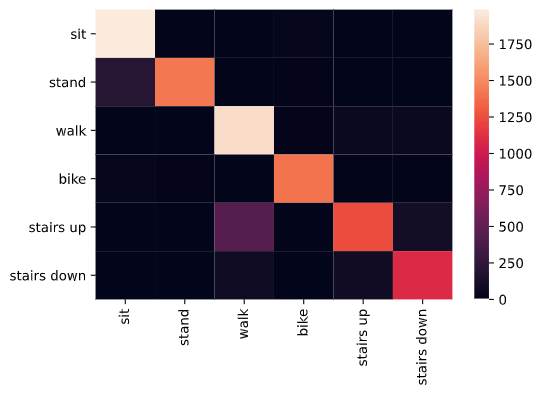
\includegraphics[width=0.5\textwidth]{images/confusion_matrix.png}
	\caption{CNN confusion matrix}
	\label{fig:cnn-confusion-matrix}
\end{figure}


\subsection{Oriented Dataset (OD)}

With this new collected dataset we want to test our model
performances in a real use case scenario, where smartphone could be
placed in different positions and orientations. In this case we
trained the model with the entire HD as training set, and then use the
OD as a test set. It is important to remember that in this case we apply OIT and so we condensed the \textit{sit} and \textit{stand} activities of HD into a one class \textit{no activity} category.

\textbf{Autoencoder.}  An interesting result, as the
Tab.~\ref{tab:ae-loss} confirms, is that OIT is a necessary operation
when dealing with HAR signals. For example, without OIT we can see
that the autoencoder trained and tested on same data goes from
$0.747241$ to $10.421337$ MSE: more than $10$ times worse. Furthermore,
data from hand or pocket-up/down do not inflate the loss too
much. This is good because it indicates that autoencoder is producing
robust features.

\begin{table}[h]
  \centering
  \begin{tabular}{lr}
    \hline
    Scenario & Loss (MSE) \\
    \hline
    HD + OIT + OD validation & 0.747241 \\
    HD + OIT + OD validation (allpos) & 0.821241 \\
    HD + OD validation & 10.421337 \\
    \hline
  \end{tabular}
  \caption{Autoencoder loss on different scenarios}
  \label{tab:ae-loss}
\end{table}

The Tab. \ref{tab:knn-metrics} and \ref{tab:ffnn-metrics} show
respectively KNN and FFNN evaluation for the best autoencoder with
$36$ features and the two classifier with hyper-parameters selected in
Sec. \ref{subsec:heterogeneity-dataset}. From this results, we can
observe that KNN is more stable and not influenced by sensor's
position/orientation w.r.t. FFNN. Also, the two models preserve evaluation order: on \textit{pouch} position gets best results on both
models, while the worse positions is \textit{hand+pocket}, as we
expect.

\begin{table}[h]
  \centering
  \begin{tabular}{lrrrr}
    \hline
    Positions & Accuracy & Precision & Recall & F1-score \\
    \hline
    Pouch & 80.1 & 86.4 & 80.7 & 79.0 \\
    Hand+Pocket & 79.5 & 83.7 & 79.5 & 79.6 \\
    All & 80.0 & 83.8 & 79.1 & 78.2 \\
    \hline
  \end{tabular}
  \caption{KNN evaluation onto OD between smartphone positions (pouch
    left/right/top/back, hand and pocket-up/down, all positions)}
  \label{tab:knn-metrics}
\end{table}

\begin{table}[h]
  \centering
  \begin{tabular}{lrrrr}
    \hline
    Positions & Accuracy & Precision & Recall & F1-score \\
    \hline
    Pouch & 74.4 & 84.7 & 74.4 & 74.8 \\
    Hand+Pocket & 67.8 & 78.0 & 67.8 & 70.0 \\
    All & 69.9 & 81.3 & 69.9 & 72.4 \\
    \hline
  \end{tabular}
  \caption{FFNN evaluation onto OD between smartphone positions (pouch
    left/right/top/back, hand and pocket-up/down, all positions)}
  \label{tab:ffnn-metrics}
\end{table}

\textbf{CNN Network.}  As reported in
Tab. \ref{tab:model-oit-performance}, we managed to get great results
also on data gathered with new sensor's position and orientation. We
noticed a performance drop of nearly $15\%$ for \textit{hand+pocket}
data, but this could be due to the CNN architecture which focus more
on the local shape and less on the real information. 

\begin{table}[h]
  \begin{center}
    \begin{tabular}{p{1.8cm}rrrr}
      \hline
      Positions & Accuracy & Precision & Recall & F1-score \\
      \hline
      Pouch & 85.3 & 92.0 & 73.8 & 81.9 \\
      Hand+Pocket & 70.5 & 79.5 & 63.0 & 70.2 \\
      All & 78.0 & 84.0 & 69.0 & 75.7 \\
      \hline
    \end{tabular}
    \caption{CNN classification comparisons onto \textit{OD} between
      smartphone positions (pouch left/right/top/back, hand and
      pocket-up/down and all positions).}
    \label{tab:model-oit-performance}
  \end{center}
\end{table}
\vspace{-0.4cm}
In conclusion, OIT turned out to be an extremely useful preprocessing
technique both for autoencoder and CNN. Without OIT, the drop for the
CNN was of nearly $45$\% for all metrics!  As Tab. \ref{tab:model-oit-performance} confirms, combining
the power of the CNN with automatically extracted features and smart
data preprocessing could lead to good results even with new problem
settings.